\begin{table*}[t]
\centering

% Keep the compact column spacing local to the tabular.
\begingroup
\setlength{\tabcolsep}{3pt}

\begin{tabularx}{\textwidth}{@{}ll*{6}{Y}@{}}

\toprule
\multirow{2}{*}{\textbf{Model}}
& \multirow{2}{*}{\textbf{Setting}}
& \multicolumn{6}{c}{\textbf{OpenVisTool-Bench}}
\\
\cmidrule(lr){3-8}

& & \textbf{Chart}
& \textbf{GUI}
& \textbf{Table}
& \textbf{VisualSearch}
& \textbf{Web2HTML}
& \textbf{AVG} \\
\midrule

\multirow{2}{*}{GPT-5.5}
& w/o tool
& 63.3
& 17.7
& 48.9
& 27.7
& 51.7
& 41.9 \\

& with tool
& \textbf{66.6}
& 24.2
& \textbf{53.9}
& 46.2
& \textbf{54.3}
& \underline{49.0} \\

\addlinespace[1pt]

\multirow{2}{*}{Kimi K2.6}
& w/o tool
& 50.9
& 17.1
& 34.4
& 13.8
& 49.4
& 37.6 \\

& with tool
& \underline{64.3}
& 18.8
& \underline{51.6}
& 49.8
& \underline{53.6}
& 45.9 \\

\midrule
Qwen2.5-VL-7B
& w/o tool
& 18.2
& 5.1
& 21.2
& 28.3
& 23.1
& 19.2 \\

\addlinespace[1pt]

Thyme
& with tool
& 19.8
& 0.0
& 17.9
& 39.2
& 14.3
& 18.2 \\

\addlinespace[1pt]

DeepEyes V2
& with tool
& 20.9
& 1.7
& 20.4
& 31.8
& 2.4
& 15.5 \\

\midrule
\multirow{2}{*}{Qwen3.5-4B}
& w/o tool
& 31.6
& 22.0
& 25.4
& 34.0
& 40.8
& 30.8 \\

& with tool
& 32.5
& 23.5
& 32.3
& 39.6
& 41.6
& 33.9 \\

\quad+\dataset
& with tool
& 43.0\imp{11.4}
& 27.4\imp{5.4}
& 37.3\imp{11.9}
& 56.6\imp{22.6}
& 43.4\imp{2.6}
& 41.5\imp{10.7} \\

\midrule
\multirow{2}{*}{Qwen3-VL-8B-Instruct}
& w/o tool
& 22.1
& 13.0
& 26.7
& 31.8
& 26.5
& 24.0 \\

& with tool
& 20.9
& 12.6
& 24.6
& 30.2
& 28.1
& 23.3 \\

\quad+\dataset
& with tool
& 26.1\imp{4.0}
& 19.7\imp{6.7}
& 35.3\imp{8.6}
& 50.7\imp{18.9}
& 32.9\imp{6.4}
& 32.9\imp{8.9} \\

\midrule
\multirow{2}{*}{Qwen3.5-9B}
& w/o tool
& 34.6
& 27.1
& 29.0
& 35.6
& 40.1
& 33.3 \\

& with tool
& 28.4
& 24.8
& 26.8
& 38.7
& 42.0
& 32.1 \\

\quad+\dataset
& with tool
& 49.3\imp{14.7}
& \textbf{31.6}\imp{4.5}
& 43.1\imp{14.1}
& \textbf{59.4}\imp{23.8}
& 45.5\imp{5.4}
& 45.8\imp{12.5} \\

\midrule
\multirow{2}{*}{Qwen3.5-27B}
& w/o tool
& 45.7
& 28.9
& 29.8
& 43.2
& 46.6
& 38.8 \\

& with tool
& 47.7
& \underline{29.1}
& 43.3
& 54.7
& 44.3
& 43.8 \\

\quad+\dataset
& with tool
& 60.7\imp{15.0}
& \textbf{31.6}\imp{2.7}
& 48.2\imp{18.4}
& \underline{57.3}\imp{14.1}
& 48.7\imp{2.1}
& \textbf{49.3}\imp{10.5} \\

\bottomrule
\end{tabularx}
\endgroup

\caption{
Main results on OpenVisTool-Bench. Qwen2.5-VL-7B-Instruct is the shared backbone of Thyme and DeepEyes V2. +OpenVisTool-42K rows use our training data, and green $+x$ suffixes show absolute gains over the no-tool baseline. Our data improves the five-domain average by 8.9--12.5 points. \textbf{Bold} and \underline{underlined} entries mark the best and second-best results.
}
\label{tab:main}

\end{table*}


\section{Experiments}
\label{sec:experiments}

We design experiments to validate our central claim—that effective visual tool use is learned from instructive trajectories rather than merely successful ones—and to answer the following questions:
\begin{itemize}
    \item \textbf{Effectiveness:} Does fine-tuning on OpenVisTool-42K teach models to effectively leverage visual tools, and can it lift open-source models to closed-source performance levels? (\S\ref{sec:main_results})
    
    \item \textbf{Generalization:} Does the learned tool-use capability transfer to out-of-distribution visual tasks unseen during training, rather than overfitting to domain-specific tool-calling patterns? (\S\ref{sec:ood})
    
    \item \textbf{Supervision verification:} Are outcome validity and causal utility both necessary for constructing effective visual tool-use supervision? (\S\ref{sec:ablation_gain})
    
    \item \textbf{Cross-domain synergy:} Does visual tool use emerge as a transferable meta-skill across domains, and does multi-domain training resolve strategy conflicts that single-domain training introduces? (\S\ref{sec:cross_domain})
\end{itemize}

\subsection{\benchname: Isolating Tool-Use Ability}
\label{sec:bench}

% We introduce \benchname, a multi-domain evaluation suite specifically designed to measure how effectively models leverage visual tools.
% Unlike existing benchmarks that conflate general visual understanding with tool-augmented reasoning, \benchname{} isolates the incremental value of active tool use by retaining only instances where tools are beneficial.
General-purpose visual benchmarks often mix tool-relevant instances with questions that can already be solved reliably from the initial image encoding. To isolate the incremental value of active tool use, we introduce \benchname, a multi-domain evaluation suite specifically designed to measure how effectively models leverage visual tools.

\paragraph{Design goal.}

\benchname targets tasks that demand active visual evidence acquisition: the information needed to answer correctly is difficult to obtain from a single static view, requiring models to interact with the visual environment (e.g., cropping into regions of interest, enhancing contrast for faint details, or detecting edges and contours to isolate structure) to gather sufficient evidence. Concretely, we retain only the instances for which tool use is clearly beneficial, rather than uniformly sampling from the source benchmarks.


\paragraph{Per-domain construction.}

The two mechanisms below differ in \emph{how} our goal is operationalized, depending on whether the source benchmark already isolates tool-demanding tasks or requires explicit filtering.

\begin{itemize}

\item \textbf{Chart and Table} --- source QA pools are dominated by tool-irrelevant questions, so we \emph{explicitly filter} for tool-decisive instances.
Concretely, we run three strong closed-source models (GPT-5.4, Gemini-3.0-Flash, Qwen3.5-Plus) on every instance under two conditions (with and without tools), each sampled five times.
An instance is retained if, for \emph{any} of the three models, the accuracy gain (avg@5\textsubscript{tool} $-$ avg@5\textsubscript{no-tool}) exceeds a threshold of 0.3, indicating that tool use provides a clear and consistent advantage.
Taking the \emph{union} across models ensures the criterion captures ``tools \emph{in principle} help'' (model-agnostic) rather than ``\emph{our} toolset helps a specific model,'' avoiding circularity with the evaluated students.
We further report results on the complete (unfiltered) Chart and Table source benchmarks in Appendix~\ref{app:fullset}; the consistent gains confirm that our filtering sharpens an existing signal rather than manufactures one.


\item \textbf{GUI, Visual Search, Web-to-HTML} --- unlike the chart/table sources, these benchmarks are \emph{already} curated around a specific visual operation (precise click localization, fine-grained visual retrieval, and faithful layout reproduction, respectively). The tasks inherently require active manipulation of the visual input, making an additional tool-gain filter unnecessary. We therefore adopt them directly: the smallest-target subset of ScreenSpot-Pro (117 items), VisualProbe-Hard, and Vision2Web-Level1.

\end{itemize}


\paragraph{Evaluation protocol.}
Each domain uses an evaluator matched to its task type.
\textbf{Chart, Table, and Visual Search}: an extraction pipeline followed by majority-vote LLM judging yields a binary ($0/1$) correctness score.
\textbf{GUI}: a prediction is correct if the predicted click coordinate falls within the ground-truth bounding box.
\textbf{Web-to-HTML}: we render the generated HTML and compute component-level visual fidelity against the reference page (scaled $0$--$100$).
We report per-domain scores and their macro-average under the avg@$k$ protocol.


\subsection{Experimental Setup}
\label{sec:setup}

\paragraph{Benchmarks.}
We primarily evaluate on \benchname, which covers diverse visual tool-use scenarios across multiple domains. To assess generalization, we additionally test on Agentic-MME and VTC-Bench. We also report results on the full Chart and Table source benchmarks to confirm that gains are not artifacts of our data filtering (Appendix~\ref{app:fullset}).

\paragraph{Baselines.}
We compare three types of models. (i)~General-purpose frontier models: GPT-5.5 and Kimi K2.6~\citep{kimik26blog}, both evaluated without tools and with our shared toolset. (ii)~Smaller-scale general-purpose models: Qwen2.5-VL-7B~\citep{Qwen2.5-VL}, Qwen3-VL-8B-Instruct~\citep{Qwen3-VL} and Qwen3.5~\citep{qwen35blog} series are evaluated both without tools and with our shared toolset before fine-tuning. (iii)~Open-source visual tool-use agents: Thyme~\citep{zhang2026thyme} and DeepEyes V2~\citep{hong2026deepeyesv2}, evaluated with the code-based tool environments used in their original work rather than our toolset.

\paragraph{Training.}
We fine-tune four base models: Qwen3.5-4B/9B/27B and Qwen3-VL-8B-Instruct. All models are trained on \dataset for 3 epochs using SWIFT~\citep{zhao2025swift}. More implementation details are provided in Appendix \ref{app:implement}.

\subsection{Main Results}
\label{sec:main_results}
Table~\ref{tab:main} summarizes performance across all models. We highlight several key findings below.

\paragraph{Consistent gains across all base models and domains.}
Our method yields substantial improvements over the no-tool baselines across all domains and model scales. Across models ranging from 4B to 27B, fine-tuning with \dataset{} brings an average gain of 10.7 points on \benchname, with the most pronounced improvement observed in VisualSearch (+23.8 points). 
Notably, even without any fine-tuning, simply equipping strong off-the-shelf models with our toolset provides significant benefits: the closed-source GPT-5.5 and the open-source Kimi K2.6 achieve 7.1 and 14.1 absolute gains, respectively, demonstrating the inherent utility of the designed tools.
However, for smaller open-source models, naively providing tools without dedicated training yields marginal or even negative returns—Qwen3.5-9B, for instance. After fine-tuning on \dataset, these same models learn to leverage tools effectively, comparable to closed-source models. For example, Qwen3.5-9B with our training achieves an average of 45.8, surpassing GPT-5.5's 41.9 without tools and closely approaching its tool-augmented performance of 49.0.
In contrast, existing tool-use models Thyme and DeepEyes V2, trained on narrow single-domain data, perform worse on the five-domain average than vanilla base models \emph{without any tool access}—they improve on their specialty but collapse catastrophically elsewhere. This comparison highlights that a diverse, multi-domain training corpus, as provided by \dataset{}, is essential for robust and generalizable visual tool use.

\paragraph{Largest gains emerge where tools unlock new visual evidence.}
For domains where the answer is largely derivable from surface-level visual content—such as Chart, which primarily tests text and semantic extraction from images—a sufficiently capable model can already perform well without tools (e.g., GPT-5.5 scores 63.3 on Chart without tools). However, for more challenging domains involving dense details and hidden evidence—such as VisualSearch, which demands fine-grained spatial and geometric reasoning—models often struggle to succeed with their inherent visual perception alone. In these scenarios, invoking auxiliary tools to crop, zoom, or reformat visual content becomes essential. This explains why our method yields the most substantial gains precisely in these demanding domains (e.g., Qwen3.5-9B: +23.8 points on VisualSearch), where tools effectively bridge the gap between what the model can perceive and what the task requires.


\subsection{Out-of-Distribution Generalization}
\label{sec:ood}

\begin{table}[t]
\centering

\begingroup
\small
\setlength{\tabcolsep}{4pt}
\begin{tabular*}{\columnwidth}{@{\extracolsep{\fill}}lcc@{}}

\toprule
\textbf{Model}
& \textbf{Agentic-MME}
& \textbf{VTC-Bench} \\
\midrule

Qwen3.5-4B
& 29.9
& 27.5 \\

\quad+\dataset
& 34.5\imp{4.6}
& 38.8\imp{11.3} \\

\midrule
Qwen3-VL-8B-Instruct
& 25.6
& 28.2 \\

\quad+\dataset
& 32.3\imp{6.7}
& 29.1\imp{0.9} \\

\midrule
Qwen3.5-9B
& 32.7
& 30.1 \\

\quad+\dataset
& \textbf{41.6}\imp{8.9}
& \underline{41.4}\imp{11.3} \\

\midrule
Qwen3.5-27B
& 37.1
& 34.9 \\

\quad+\dataset
& \underline{41.1}\imp{4.0}
& \textbf{45.2}\imp{10.3} \\

\bottomrule
\end{tabular*}
\endgroup

\caption{
Out-of-distribution results on Agentic-MME and VTC-Bench. Untrained backbones are evaluated without tools, while +OpenVisTool-42K models are evaluated with tools. Green $+x$ suffixes show absolute gains over the corresponding no-tool backbone. \textbf{Bold} and \underline{underlined} entries mark the best and second-best results.
}
\label{tab:ood}

\end{table}


To test whether the tool-use capability learned from our five training domains transfers beyond them, we further evaluate on Agentic-MME and VTC-Bench with out-of-distribution domains held out from training. Table~\ref{tab:ood} directly compares each off-the-shelf backbone with its \dataset-trained counterpart, with tools enabled for every model. Training improves all four backbones on both benchmarks, by 1.3--7.9 points on Agentic-MME and 3.9--17.6 points on VTC-Bench. Notably, Qwen3.5-9B rises from 23.8 to 41.4 on VTC-Bench after training. These gains indicate that \dataset teaches a transferable tool-use policy rather than a domain-specific invocation pattern.

\begin{figure}[t]
    \centering
    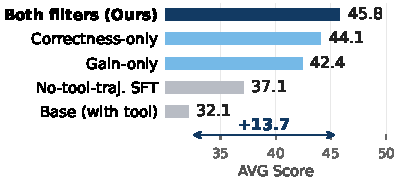
\includegraphics[width=0.9\columnwidth]{figures/fig_ablation.pdf}
    % \caption{Comparison of training variants.}
    \caption{Ablation of the criteria for instructive tool-use supervision on Qwen3.5-9B under a fixed training budget. Requiring both outcome validity and causal utility achieves the best performance, outperforming either criterion alone and the no-tool-trajectory SFT baseline.}
    \label{fig:ablation}
\end{figure}

\begin{table}[t]
    \centering
    \small
    \setlength{\tabcolsep}{3.5pt}
    \begin{tabular}{@{}lccc@{}}
    \toprule
    \textbf{Trajectory source} & \textbf{\shortstack{OpenVisTool-\\Bench}} & \textbf{\shortstack{Agentic-\\MME}} & \textbf{\shortstack{VTC-\\Bench}} \\
    \midrule
    None (Qwen3.5-9B w/o tool) & 33.3 & 32.7 & 30.1 \\
    Correctness-only model & 42.1 & 36.5 & 36.5 \\
    Instructive model (ours) & \textbf{44.5} & \textbf{37.7} & \textbf{38.1} \\
    \bottomrule
    \end{tabular}
    \caption{Trajectory replay analysis using the original Qwen3.5-9B probe model. The probe model answers each query conditioned on the tool call arguments and returned observations generated by the correctness-only or instructively trained model. The generator's reasoning and final answer are excluded. ``None'' denotes evaluation without tool access or trajectory replay.}
    \label{tab:trajectory_replay}
\end{table}


\subsection{Ablation Study}
\label{sec:ablation_gain}
\label{sec:notool_traj}
To validate that effective visual tool-use learning requires both correct answers and causally useful tool traces, we compare four Qwen3.5-9B supervision variants under the same training budget. The first three use tool trajectories retained by (1)~both outcome validity and causal utility (full \dataset{}), (2)~outcome validity alone, or (3)~causal utility alone. The fourth is a no-tool-trajectory SFT baseline, constructed by re-synthesizing trajectories without tool invocation for the queries in the full variant.


\paragraph{Gains originate from tool-use, not from SFT alone.}
As shown in Figure~\ref{fig:ablation}, every tool-augmented variant outperforms the no-tool-trajectory SFT baseline, confirming that improvements stem from learned tool invocation rather than simply training on additional difficult queries.


\paragraph{Both filters are complementary and necessary.}
Intersecting both filters consistently dominates either filter in isolation, with outcome-validity-only and causal-utility-only trailing by 1.7 and 3.4 points, respectively.
The two filters address distinct failure modes: outcome validity removes demonstrations that lead to incorrect answers and would teach erroneous behavior, while causal utility discards trajectories where tools are invoked but their observations contribute no measurable benefit to reaching the solution. Their combination yields the highest-quality training signal.


\paragraph{Instructive filtering yields more useful tool interactions.}
To probe the learned behavior beyond the accuracy of the fine-tuned models themselves, we replay their tool-interaction trajectories to the original Qwen3.5-9B probe model. The replayed context contains only tool call arguments and returned observations; all reasoning and final answers from the trajectory-generating model are excluded, ruling out direct copying of the generator's answer or imitation of its rationale. As shown in Table~\ref{tab:trajectory_replay}, trajectories from both trained models improve the base model on all three benchmarks, but those from the instructively trained model consistently outperform correctness-only trajectories. This behavior-level transfer suggests that causal-utility filtering induces an evidence-acquisition policy whose resulting interactions are more useful to another model, rather than merely producing tool calls that accompany successful outcomes.

\begin{table*}[t]
\centering
\small

\begin{tabular}{llcccccc}
\toprule
\textbf{Variant} & \textbf{Setting} & \textbf{Chart} & \textbf{GUI} & \textbf{Table} & \textbf{VisualSearch} & \textbf{Web2HTML} & \textbf{AVG} \\
\midrule
\multirow{2}{*}{Qwen3.5-9B} & w/o tool & 34.6 & 27.1 & 29.0 & 35.6 & 40.1 & 33.3 \\
 & with tool & 28.4 & 24.8 & 26.8 & 38.7 & 42.0 & 32.1 \\
\midrule
+ \dataset{} (full) & with tool & \textbf{49.3} & \underline{31.6} & \textbf{43.1} & \textbf{59.4} & \textbf{45.5} & \textbf{45.8} \\
\midrule
\multicolumn{8}{l}{\textit{Single-domain slices}} \\
\quad + Chart & with tool & \underline{46.6} & 22.2 & 37.1 & 44.3 & 36.5 & 37.4 \\
\quad + GUI & with tool & 41.4 & \textbf{36.3} & 38.7 & 52.8 & 39.1 & \underline{41.7} \\
\quad + Table & with tool & 45.7 & 20.5 & \underline{38.9} & 45.8 & 39.2 & 38.0 \\
\quad + VisualSearch & with tool & 45.7 & 23.3 & 40.9 & \underline{57.3} & 21.6 & 37.8 \\
\quad + Web2HTML & with tool & 41.6 & 18.2 & 38.5 & 42.2 & \underline{44.6} & 37.0 \\
\bottomrule
\end{tabular}

\caption{Cross-domain transfer with Qwen3.5-9B. We fine-tune the model on either the full \dataset{} mixture or an individual domain slice and evaluate all fine-tuned variants with tools across the five domains.}
\label{tab:cross}

\end{table*}


\subsection{Cross-Domain Transfer}
\label{sec:cross_domain}

% \paragraph{Setup.}
We fine-tune Qwen3.5-9B on each single-domain slice of \dataset{} separately and evaluate on all five domains. Full results are reported in Table~\ref{tab:cross}.

\paragraph{Tool-use transfers as a domain-general meta-skill.}
Training on any single domain improves overall performance over the tool-enabled base model, with gains often extending to domains unseen during training. Most notably, GUI-only training improves VisualSearch by 14.1 points. This cross-domain benefit suggests that the model learns reusable tool-use primitives, such as localized cropping and spatial grounding, rather than only domain-specific solutions.

\paragraph{Transfer is asymmetric, with both positive and negative effects.}
The transfer is not uniformly beneficial because different domains reward different interaction patterns. For example, VisualSearch-only training lowers Web2HTML performance from 42.0 to 21.6. We attribute this degradation to a mismatch in tool-use strategies: repeatedly cropping small regions is effective for fine-grained search but conflicts with the global, full-page reasoning. Single-domain training can therefore over-specialize the tool-use policy and harm domains that require incompatible strategies.

\paragraph{The full mixture resolves strategy conflicts.}
The full \dataset{} mixture achieves a 45.8 average, surpassing all single-domain variants, and performs best on four of the five domains. Exposure to diverse interaction patterns helps the model resolve strategy conflicts through \emph{context-conditional} tool use: it learns not only how to invoke tools, but also which strategy is appropriate for the visual input.

\paragraph{The GUI exception.}
GUI is the only domain where a specialist trained on its single-domain slice outperforms the full mixture on the corresponding domain. A likely reason is that the point-in-bbox metric rewards a single precise click, making direct imitation especially effective, whereas other domains emphasize multi-step interactions such as crop$\to$OCR. Because the full mixture still improves GUI over the untuned tool-enabled base model, this exception points to domain-adaptive mixture weighting rather than a failure of multi-domain tool-use supervision.
